\documentclass[UTF8, a4paper, linespread=1.5]{article}

\usepackage{tcolorbox, listings, algorithm, minted, algpseudocode}
\usepackage{geometry, savesym, amsmath, enumerate, indentfirst, color, amsthm, bm, extarrows, ulem}
\usepackage{amssymb}
\usepackage{nameref, hyperref}
 \geometry{top=3cm, bottom=3cm, left=1.5cm, right=1.5cm}

\usepackage{enumitem}
\setenumerate[1]{itemsep=0pt,partopsep=0pt,parsep=\parskip,topsep=5pt}
\setitemize[1]{itemsep=0pt,partopsep=0pt,parsep=\parskip,topsep=5pt}

\renewcommand\contentsname{Contents}

\tcbuselibrary{skins, breakable, theorems}

% \setlength{\leftskip}{10pt}
\setlength{\parindent}{10pt}
% \setlength{\parskip}{2em}
\renewcommand{\baselinestretch}{1.3}

\newcounter{RomanNumber}
\newcommand{\mrm}[1]{(\setcounter{RomanNumber}{#1}\Roman{RomanNumber})}

\newtcbtheorem{thm}{}
  {enhanced, theorem name and number, code={\edef\@currentlabelname{#2}}, 
  frame code={
        % \path[thick, draw] (frame.north west) -| (frame.north east) -| (frame.south east) -| (frame.south west) -| (frame.north west);
        \path[thick, draw] (frame.north west)  +(.5\baselineskip,0) -| +(0,-.5\baselineskip);
        % \path[thick, draw] (frame.north east) +(-.5\baselineskip,0) -| +(0,-.5\baselineskip);
        % \path[thick, draw] (frame.south west) +(.5\baselineskip,0) -| +(0,.5\baselineskip);
        \path[thick, draw] (frame.south east) +(-.5\baselineskip,0) -| +(0,.5\baselineskip);
    },
    left=1mm, right=1mm, top=1mm, bottom=1mm,
    colback=black!5,
    colframe=red!75!black,
    colbacktitle=black!0,
    coltitle=black!100,
    fonttitle=\bfseries}{thm}


\usepackage{environ}
\RenewEnviron{math}{%
\begin{align*}
\BODY
\end{align*}
}

\title{CS217 -- Algorithm Design and Analysis \\ Homework 5}
\date{\today}
\author{Not Strong Enough}



\begin{document}

    A \textit{multigraph} is a graph that can have multiple edges, called ``parallel edges''. Without defining it formally, we illustrate it:
    \begin{center}
        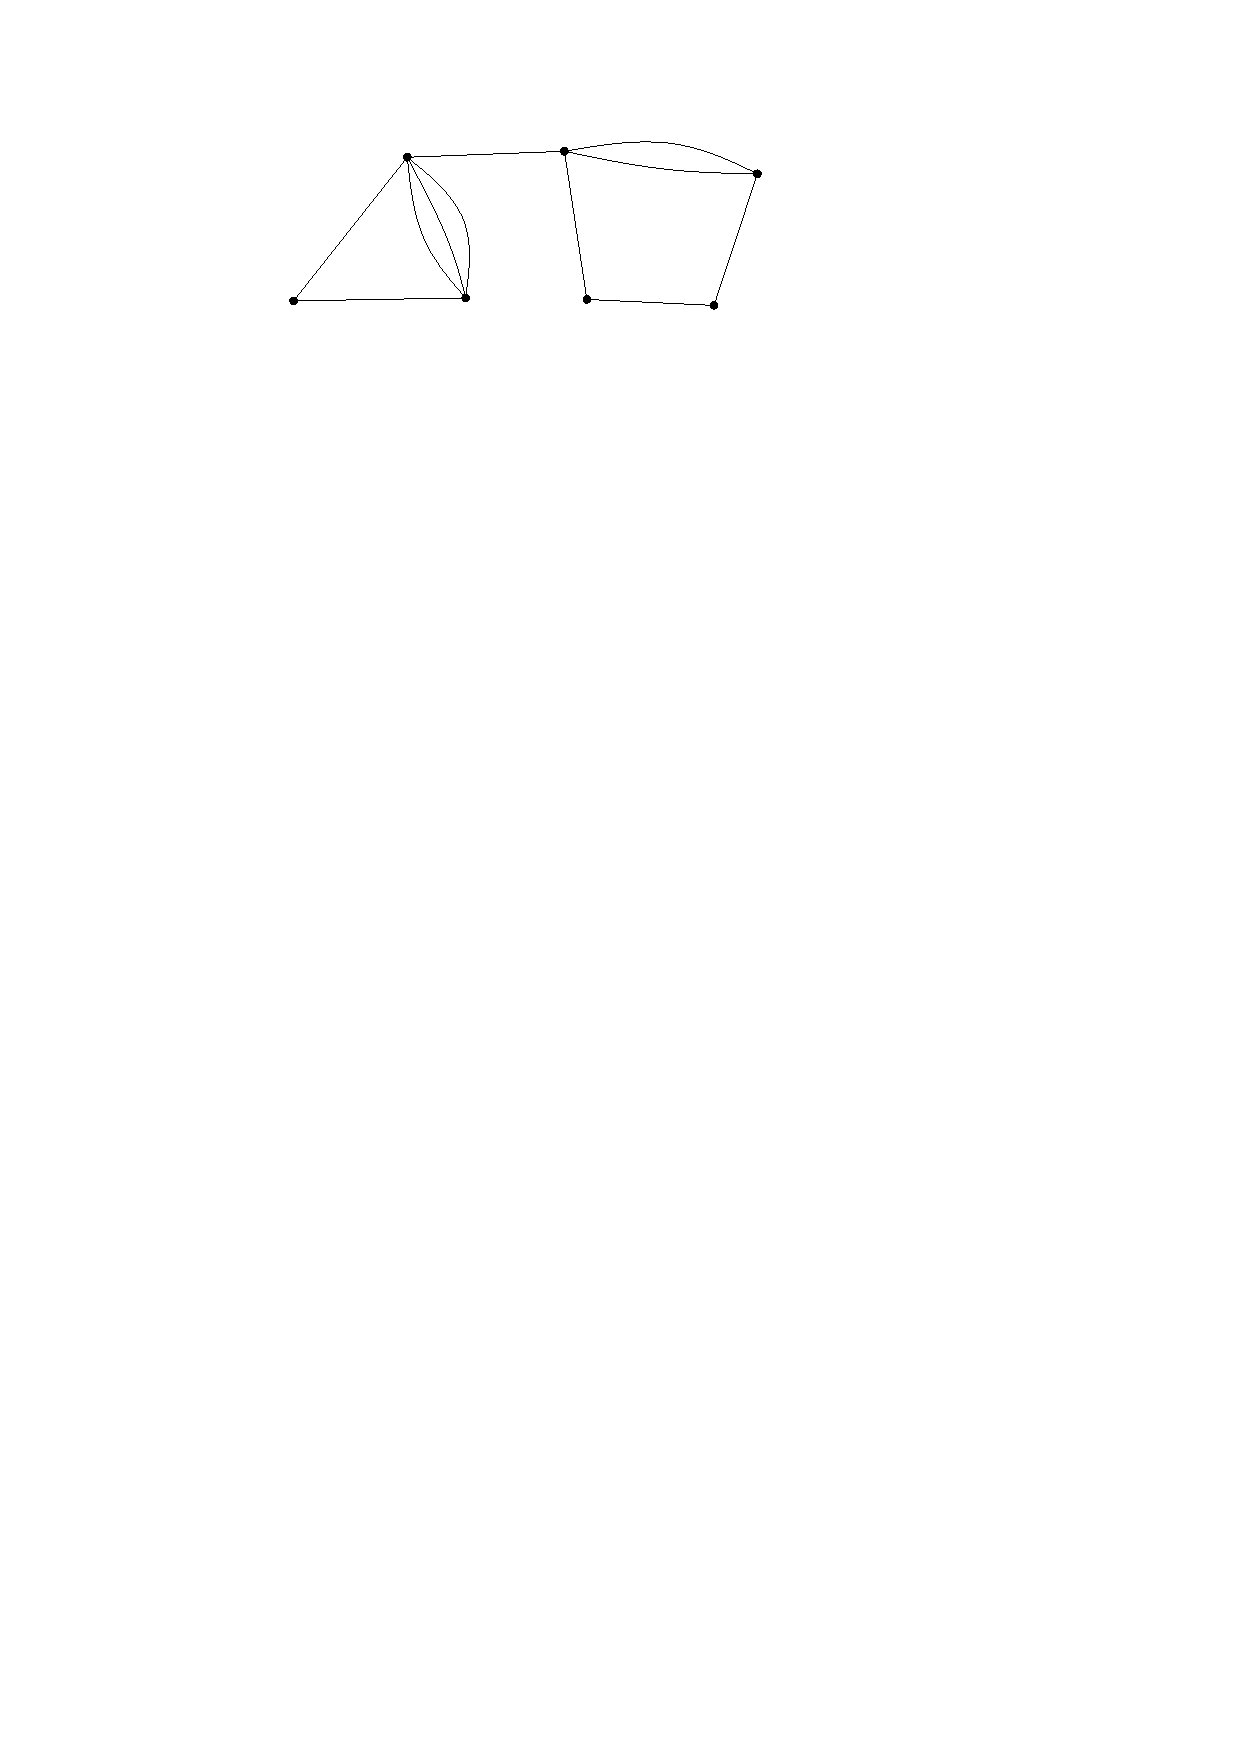
\includegraphics[width=0.4\textwidth]{figures/multigraph.pdf}\\
        A multigraph.
    \end{center}
    All other definitions, like connected components and spanning trees are the same as for normal (simple) graphs. However, when two spanning trees use different parallel edges, we consider them different:
    \begin{center}
        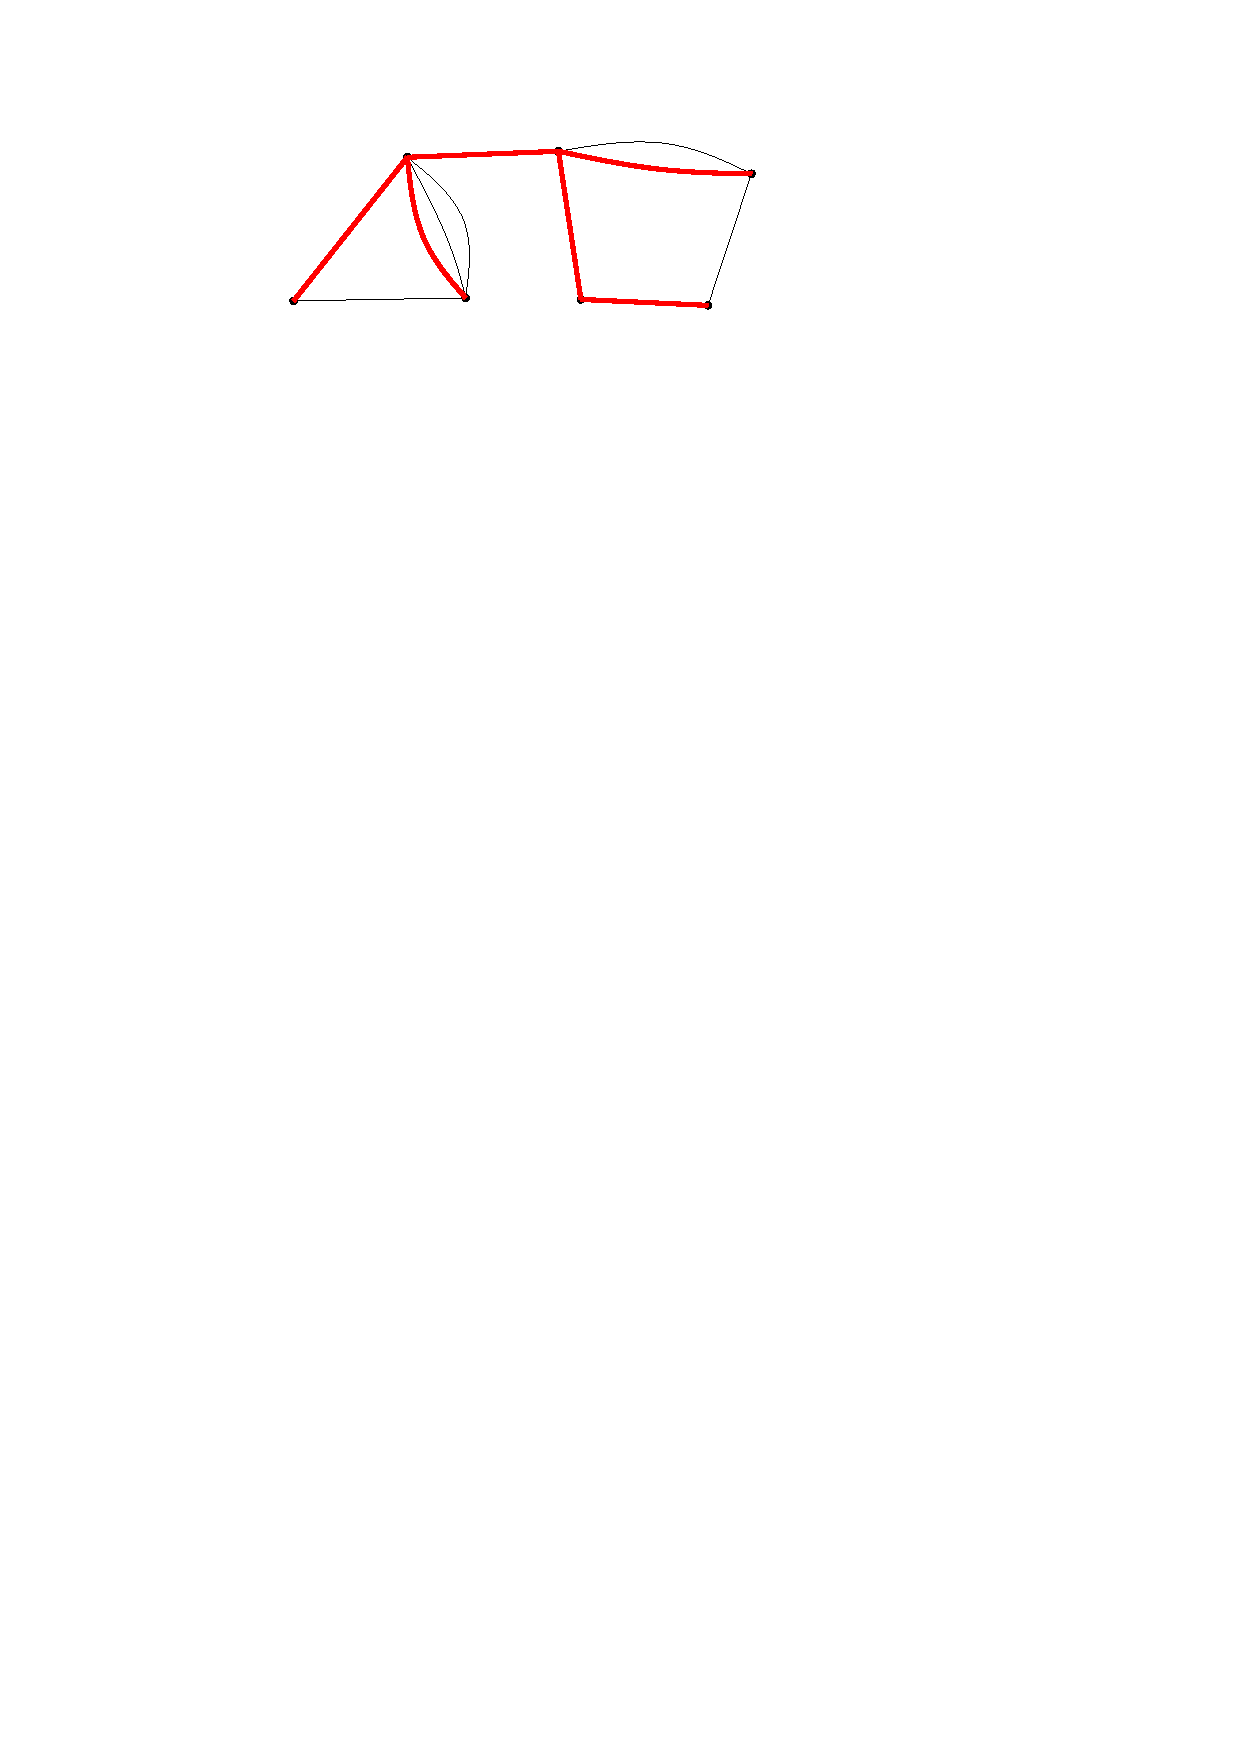
\includegraphics[width=0.3\textwidth]{figures/multigraph-forest.pdf} \hspace{2cm}
        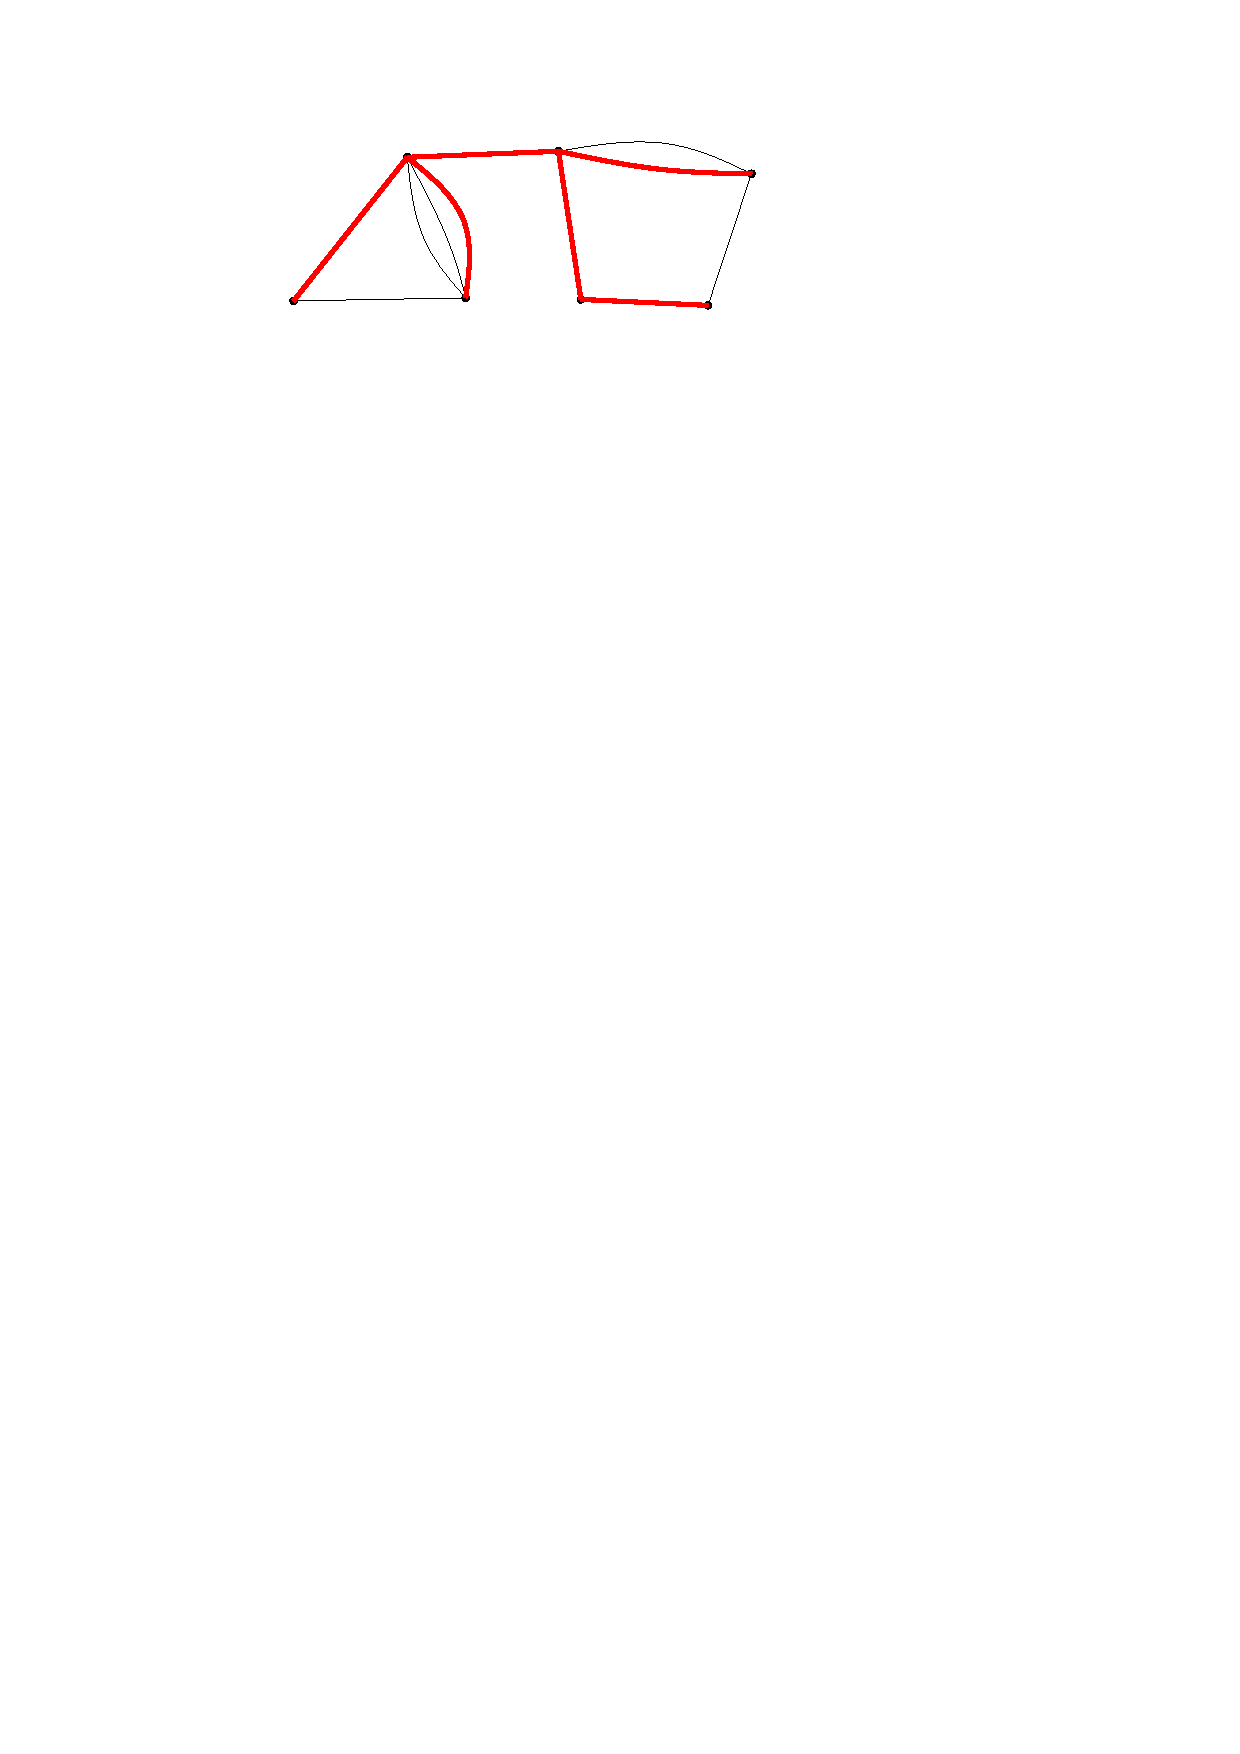
\includegraphics[width=0.3\textwidth]{figures/multigraph-forest-other.pdf} \\
        The same multigraph with two different spanning trees.
    \end{center}

    \begin{thm}{}{}
        How many spanning trees does the above multigraph on 7 vertices have? Justify your answer!
    \end{thm}

    \begin{proof}[Solution]
        Firstly, we label the 7 vertices from $a$ to $g$ as below.
        \begin{center}
            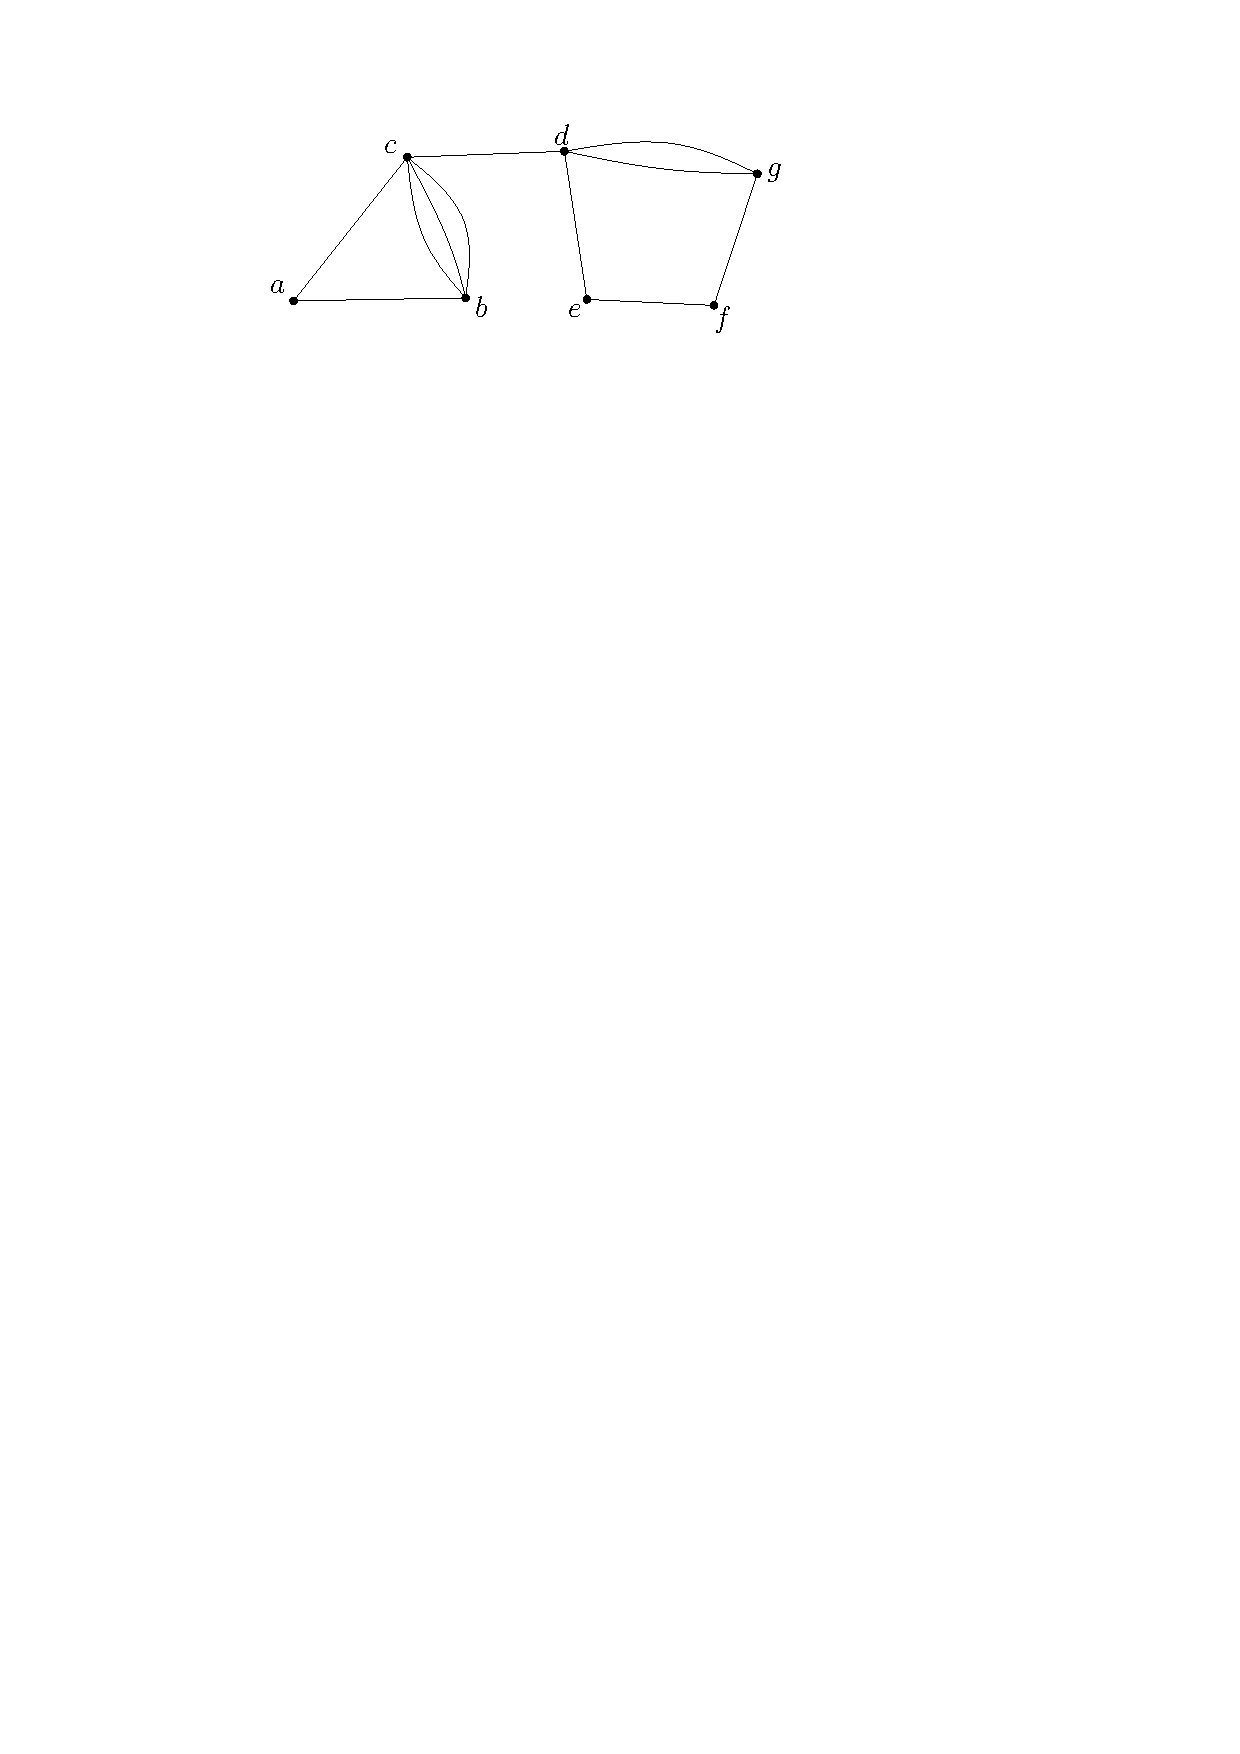
\includegraphics[width=0.4\textwidth]{figures/multigraph-labeled.pdf}
        \end{center}
    
        Obviously, as a bridge, the edge $\{c, d\}$ is contained in every spanning tree. So we only need to count the number of spanning trees of vertices $V_1 = \{a, b, c\}$ and $V_2 = \{d, e , f, g\}$ respectively, and then multiplying the two numbers we get the number of spanning trees of the original graph.
        \begin{center}
            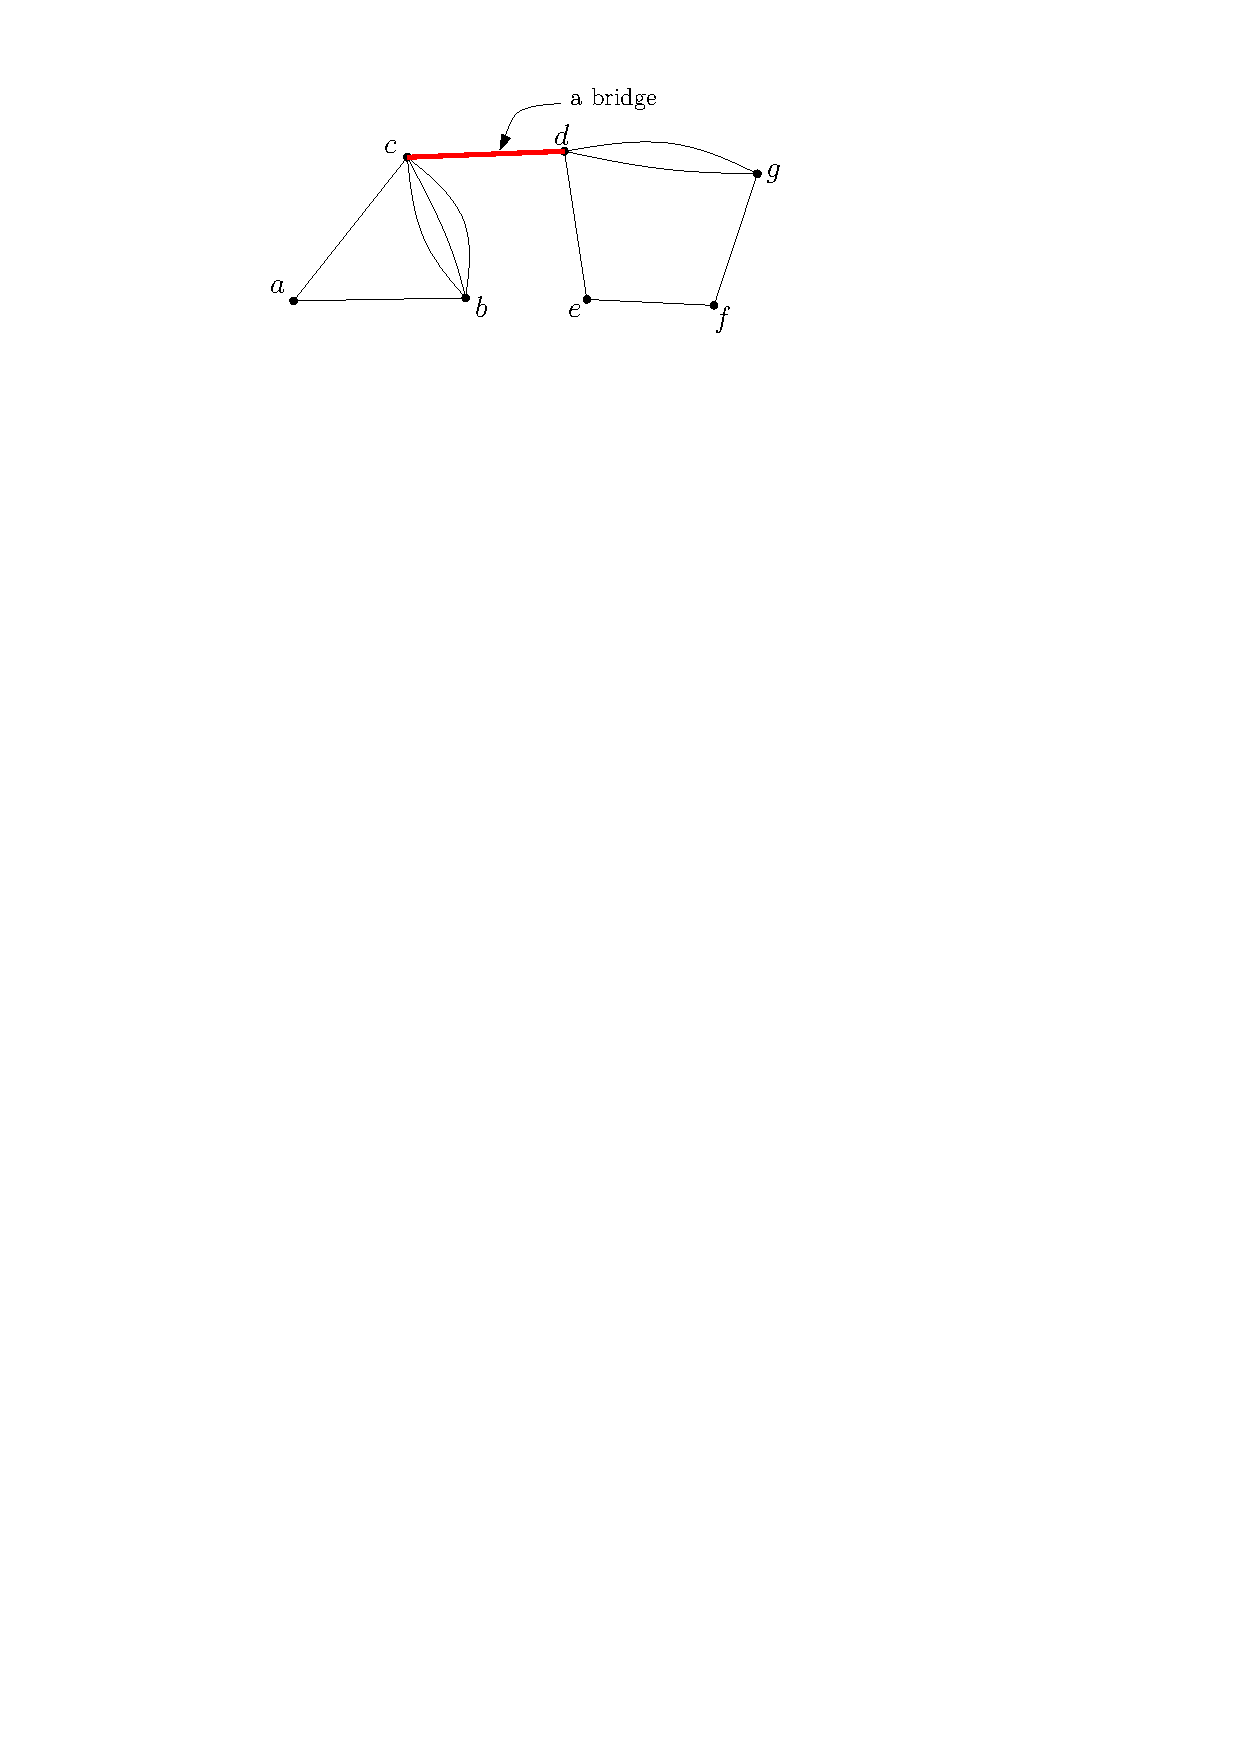
\includegraphics[width=0.4\textwidth]{figures/multigraph-bridge.pdf}
        \end{center}
        
        Consider the sub-multigraph with vertices $a$, $b$ and $c$. If we select none of the edges between $b$ and $c$, there are only $1$ spanning tree. Otherwise we select one of the edges between $b$ and $c$, and we can select another edge which is either $\{a, c\}$ or $\{a, b\}$. So there are $cnt_l = 1 + 2 \times 3 = 7$ spanning trees in the left sub-multigraph.
        
        Then we consider the right sub-multigraph with vertices $d$ to $g$. Similarly, there is only one spanning tree which doesn't contain an edge between $d$ and $g$. And if we select an edge between $d$ and $g$, the other two edges can be any two among $\{d, e\}$, $\{e, f\}$ and $\{f, g\}$. So there are $cnt_r = 1 + 3 \times 2 = 7$ spanning trees in the right sub-multigraph.
        
        Finally we multiply $cnt_l$ and $cnt_r$. So the total number of spanning trees in the given multigraph is $cnt_l \times cnt_r = 7 \times 7 = 49$.
    \end{proof}


\end{document}

